
%(BEGIN_QUESTION)
% Copyright 2006, Tony R. Kuphaldt, released under the Creative Commons Attribution License (v 1.0)
% This means you may do almost anything with this work of mine, so long as you give me proper credit

Determine a basic 5-point (0\%, 25\%, 50\%, 75\%, and 100\%) calibration table for the displacer level transmitter in this scenario:

$$\includegraphics[width=15.5cm]{i00279x01.eps}$$

The cylindrical displacer weighs 15 pounds (dry) and has a diameter of 3.5 inches.  The process liquid has a density of 55 lb/ft$^{3}$.  The 0\% process liquid level (LRV) is even with the bottom of the displacer.  Assume an electronic transmitter mechanism with an output range of 4 to 20 mA, and a calibration tolerance of +/- 0.2\% (of span).

% No blank lines allowed between lines of an \halign structure!
% I use comments (%) instead, so that TeX doesn't choke.

$$\vbox{\offinterlineskip
\halign{\strut
\vrule \quad\hfil # \ \hfil & 
\vrule \quad\hfil # \ \hfil & 
\vrule \quad\hfil # \ \hfil & 
\vrule \quad\hfil # \ \hfil & 
\vrule \quad\hfil # \ \hfil & 
\vrule \quad\hfil # \ \hfil \vrule \cr
\noalign{\hrule}
%
% First row
Process & Percent of & Buoyant & Output signal & Output signal & Output signal \cr
%
% Another row
level (in) & span (\%) & force (lb) & ideal (mA) & min. (mA) & max. (mA) \cr
%
\noalign{\hrule}
%
% Another row
  & 0 &  &  &  &  \cr
%
\noalign{\hrule}
%
% Another row
  & 25 &  &  &  &  \cr
%
\noalign{\hrule}
%
% Another row
  & 50 &  &  &  &  \cr
%
\noalign{\hrule}
%
% Another row
  & 75 &  &  &  &  \cr
%
\noalign{\hrule}
%
% Another row
  & 100 &  &  &  &  \cr
%
\noalign{\hrule}
} % End of \halign 
}$$ % End of \vbox

\underbar{file i00279}
%(END_QUESTION)





%(BEGIN_ANSWER)

% No blank lines allowed between lines of an \halign structure!
% I use comments (%) instead, so that TeX doesn't choke.

$$\vbox{\offinterlineskip
\halign{\strut
\vrule \quad\hfil # \ \hfil & 
\vrule \quad\hfil # \ \hfil & 
\vrule \quad\hfil # \ \hfil & 
\vrule \quad\hfil # \ \hfil & 
\vrule \quad\hfil # \ \hfil & 
\vrule \quad\hfil # \ \hfil \vrule \cr
\noalign{\hrule}
%
% First row
Process & Percent of & Buoyant & Output signal & Output signal & Output signal \cr
%
% Another row
level (in) & span (\%) & force (lb) & ideal (mA) & min. (mA) & max. (mA) \cr
%
\noalign{\hrule}
%
% Another row
0 & 0 & 0 & 4 & 3.968 & 4.032 \cr
%
\noalign{\hrule}
%
% Another row
7.5 & 25 & 2.297 & 8 & 7.968 & 8.032 \cr
%
\noalign{\hrule}
%
% Another row
15 & 50 & 4.593 & 12 & 11.968 & 12.032 \cr
%
\noalign{\hrule}
%
% Another row
22.5 & 75 & 6.890 & 16 & 15.968 & 16.032 \cr
%
\noalign{\hrule}
%
% Another row
30 & 100 & 9.187 & 20 & 19.968 & 20.032 \cr
%
\noalign{\hrule}
} % End of \halign 
}$$ % End of \vbox


%(END_ANSWER)





%(BEGIN_NOTES)


%INDEX% Calibration: table, level transmitter
%INDEX% Measurement, level: calibration table
%INDEX% Measurement, level: displacer (buoyancy)

%(END_NOTES)


